\begin{flushleft}
    \begin{description}
        \item[Docker:]\hfill\\
        Software für die Container Verwaltung.

        \item[ROS:]\hfill\\
        Das Acronym ROS steht für Robot Operating System, es bietet eine Sammlung von Software-Bibliotheken, Werkzeugen und ein Framework um die Softwareentwicklung und Ausführung von Andwendugen für Roboter zu erleichtern.

        Der Kern von ROS besteht aus Interfaces, genannt ROS-Graph, die eine anonymisierte und standardisierte Interprozesskommunikation ermöglichen.
        Dieser Graph ist ein Netzwerk aus 'nodes', welche über 'topics' miteinander kommunizieren.
        Auf einem 'topic' wird immer dieselbe 'message' mit einem definierten Datentyp von Nodes verbreitet. 
        Für das Verbreiten und Empfangen von Messages müssen die Nodes 'publisher' und 'subscriber' implementieren.

        Des weiteren gibt es noch viele Tools, die beispielsweise Daten visualisieren können, und eine große Menge an Bibliotheken, welche Standard-Algorithmen der Robotik implementieren.
        Diese Tools und Bibliotheken werden ebenfalls zu ROS gezählt weshalb ROS als mehr als ein Framework angesehen wird und den Titel 'Operating-System' im Namen trägt.

        Es gibt eine ältere Version von ROS die einfach nur ROS genannt wird und eine neuere Version namens ROS2.
        Der Hauptunterschied zwischen ROS und ROS2 ist, dass ROS einen zentralen Server, genannt 'ROS-Master' verwendet über den die Kommunikation abläuft und ROS2 einen dezentralen Ansatz verfolgt.
        
        ROS2 baut auf dem Data-Distribution Service Standard von OMG auf. 
        Das ist eine Spezifikation für eine Middleware, welche ein 'Data-Centric Subscriber-Publisher (DCPS)'-Modell beschreibt.


        \item[React:]\hfill\\
        Web Frontend Framework was ursprünglich von Facebook ins leben gerufen wurde.

        \item[Arduino:]\hfill\\
        Entwicklungsplatform auf Basis von Atmel AtMega Prozessoren. Wurde entworfen um Leien den Einstieg in die Microcontroller
        Welt stark zu vereinfachen. Findet heutzutage Weltweit Anwendung in der Maker Szene.

        \item[ESP32:]\hfill\\
        ESP32 bezeichnet eine Microntroller Familie auf Basis der ARM Architektur.
        Ursprünglich wurde der ESP32 von Expresif entworfen und gefertigt.

        \item[RaspberryPi:]\hfill\\
        
        \item[Toolchain:] \hfill\\
        Als Toolchain wird die Kombination von Micro-ROS und ESP-IDF bezeichnet.
        Mit Hilfe dieser beiden Frameworks wurde die Firmware für unseren Roboter programmiert und kompiliert.

        \item[RTOS]\hfill\\
        Abkürzung für Real Time Operating System. 
        In diesem Projekt wurde in erster Linie das RTOS 'FreeRTOS' verwendet, das für die Verwendung mit Mikrocontrollern optimiert ist.
        
        \item[Micro-ROS]\hfill\\
        Micro-ROS ist eine Kombination von einem RTOS, einer Client-Bibliothek, einer Middleware und einem sogenannten ROS2 Agent, 
        die Mikrocontroller möglichst effizient in das ROS-Oekosystem einbinden soll.
        
        Mit Micro-ROS ist es nicht möglich ROS-messages direkt im Netzwerk zu versenden und mit anderen Teilnehmern direkt in Verbindung zu stehen.
        Die dafür benötigte Middleware würde zu viele Ressourcen auf einem Mikrocontroller verbrauchen. 
        Stattdessen gibt es einen sogenannten ROS-Agent, mit dem sich der Mikrocontroller mit Hilfe einer für Mikrocontroller optimierten Middleware verbindet.
        Der ROS-Agent ist dann im Prinzip eine Brücke zwischen den verschiedenen Middlewares. Entsprechend muss der Agent auch auf leistungsfähigerer Hardware ausgeführt werden.    

        \begin{figure}[h!]
            \centering
            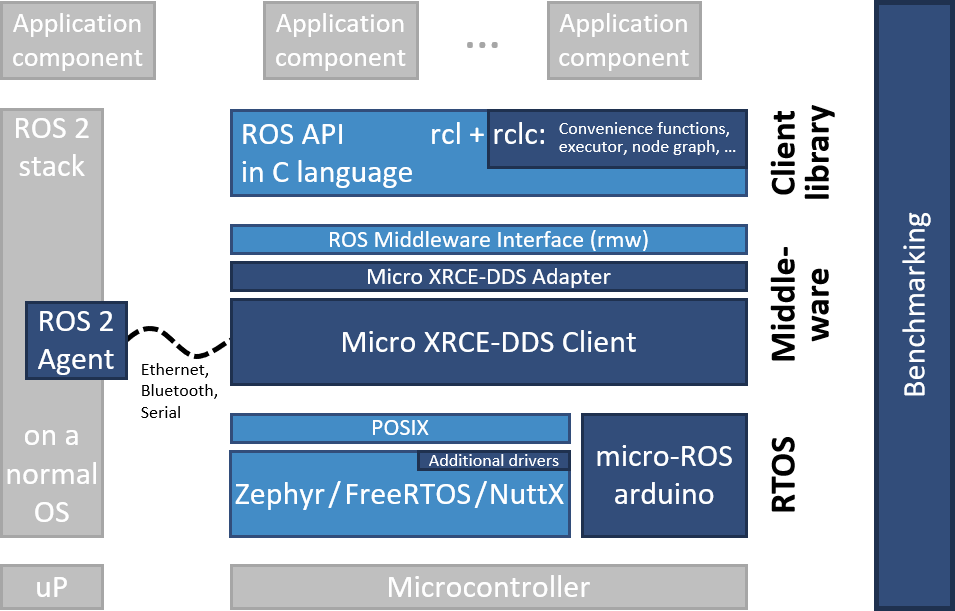
\includegraphics[width=0.8\textwidth]{imgs/Grundbegriffe/micro-ROS_architecture.png}
            \caption{Micro-ROS Architektur}
            \label{fig:micro-ros-architecture}%
        \end{figure}

        \item[ESP-IDF]\hfill\\
        ESP-IDF steht für Espressif IOT Development Framework. Das ist ein Framework mit dessen Hilfe man ESP-Socs programmieren kann.
        Das betrifft in dem Fall dann auch den ESP32.

        \end{description}
\end{flushleft}